\section{Benchmark and Method}
\subsection{Task-level mission model}
At each time step, each service can receive an arrival. An admitted mission is represented by
\begin{equation}
 m=(s,a,t_{\mathrm{arr}},t_{\mathrm{dl}},n_{\mathrm{det}}),
\end{equation}
where $s$ is the service, $a\in\{0,\ldots,4\}$ is its azimuth sector, and the deadline is at most six steps after arrival. A mission succeeds when the radar team obtains one detection with the exact $(s,a)$ identity before the deadline. The tracker credits the oldest incomplete mission with the matching service and bearing; detections at the deadline are processed before finalization. The mission drop ratio counts timeouts, admission rejects, and horizon failures over eligible missions:
\begin{equation}
 \dropRatio=\frac{N_{\mathrm{to}}+N_{\mathrm{rej}}+N_{\mathrm{hz}}}{N_{\mathrm{elig}}}.
\end{equation}
A larger value means that the jammer team denied more missions. We retain completed-but-not-yet-finalized missions in the queue, which makes the deadline accounting explicit and auditable.

\subsection{Bearing-aware link physics}
Each agent selects a beam from a $5\times5$ azimuth--elevation grid. A jammer selects a Bernoulli mask over 25 array cells and a categorical beam. For a steering direction $(u_b,v_b)$ and target $(u_t,v_t)$, the normalized planar-array response is separable and follows the standard uniform-planar-array power pattern for a $5\times5$ element grid:
\begin{align}
 G_{\mathrm{AF}}(b,t)=\;&10\log_{10}\!\left(\frac{A_{5}(u_t-u_b)^2}{5^2}\right)\nonumber\\
 &+10\log_{10}\!\left(\frac{A_{5}(v_t-v_b)^2}{5^2}\right),
\end{align}
where $A_5$ is the finite-array element factor response evaluated with the same float32 implementation for all experiments; the separable form is the usual product of azimuth and elevation linear-array factors \cite{skolnik2008,vantrees2002}. For jammer $k$ and radar $r$, the received JNR includes jammer cell aggregation, transmit and receive array gains at their pair bearing, service-dependent path loss and receiver gain, and polarization loss. Independent jammers are combined as incoherent power:
\begin{equation}
 \label{eq:jnrsum}
 \jnr_r=10\log_{10}\sum_k10^{\jnr_{kr}/10}.
\end{equation}
The effective SNR is
\begin{equation}
 \snr_{\mathrm{eff},r}=10\log_{10}\left(\frac{10^{\snr_0/10}}{1+10^{\jnr_r/10}}\right)+G_{\mathrm{coh}},
\end{equation}
with the idle case defined by $\jnr_r=-\infty$. A mission at azimuth $a$ is detected with
\begin{equation}
 p_{r}(s,a)=\sigma\left(\frac{\snr_{\mathrm{eff},r}+G_{\mathrm{target}}(b_r,a)-\tau}{w}\right),
\end{equation}
where $\tau=15$ dB and $w=3$ dB. This couples radar pointing to both useful detection gain and exposure to interference.

Table~\ref{tab:linkbudget} lists the complete link-budget parameterization. The per-pair received JNR follows the standard one-way interference budget $\jnr_{kr}=P_{\mathrm{tx}}+G_{\mathrm{tx}}+G_{\mathrm{rx}}-L_{\mathrm{path}}-L_{\mathrm{pol}}+10\log_{10}(\text{spectral overlap})-N$ with free-space path loss $L_{\mathrm{path}}=20\log_{10}(4\pi d/\lambda)$ and noise $N=-174+10\log_{10}B+\mathrm{NF}$~\cite{neri2006book}; it omits atmospheric and rain terms, which are small at X-band over 8~km relative to the dB-scale margins studied here.

\begin{table}[t]
\caption{Link-budget and detection parameters.}
\label{tab:linkbudget}
\centering
\footnotesize
\setlength{\tabcolsep}{4pt}
\begin{tabular}{ll}
\toprule
Parameter & Value \\
\midrule
Service 0 & $f_c=10.0$ GHz, $B=10$ MHz, $G_{\mathrm{rx}}=35$ dB \\
Service 1 & $f_c=10.5$ GHz, $B=20$ MHz, $G_{\mathrm{rx}}=30$ dB \\
Jammer power per cell & $P_{\mathrm{jam}}=0.1$ W \\
Jammer Tx gain & 20 dB \\
Jammer--radar range & $d=8$ km (floor 100 m) \\
Polarization loss & 3 dB \\
Noise figure & 5 dB \\
Coherent gain & $G_{\mathrm{coh}}=20$ dB \\
Baseline SNR & $\snr_0=12$ dB \\
Threshold / width & $\tau=15$ dB, $w=3$ dB \\
\bottomrule
\end{tabular}
\end{table}

Two combining assumptions deserve justification. First, \emph{within} one jammer, active cells are aggregated with phase-aligned contributions, i.e., the cell mask acts as idealized transmit beamforming; this isolates the scheduling question (which cells, which beam) from array calibration error. Second, \emph{across} jammers, received powers are summed incoherently in~(\ref{eq:jnrsum}). The two jammer sites are separated by a baseline of approximately $2d\sin 60^\circ\approx13.9$~km, i.e., about $5\times10^5$ wavelengths at 10~GHz; without phase coordination at that scale, the received phase difference is uniformly uncertain, so expected received powers---not fields---add. Coherent cross-jammer combining would require phase synchronization far beyond the threat model assumed here and would only strengthen the attacker; the incoherent model is therefore the conservative choice for the defense-side conclusions. The jamming waveform is broadband noise with rectangular spectra, so service-dependent rejection enters only through the spectral-overlap factor; we do not model pulse-to-pulse agility, Doppler, or MTI filtering, and Section~VII discusses this boundary.

\subsection{S6 and S7 games}
S6 uses one jammer against two co-located learned radar heads. S7 uses two parameter-shared jammers at azimuths $+60^\circ$ and $-60^\circ$ and two radar heads at $+20^\circ$ and $-20^\circ$. Both stages use the validated $\snr_0=12$ dB regime and $P_{\mathrm{jam}}=0.1$ W per active cell. The S7 team receives a total 63-token budget, split 32/31 between jammers; the S6-to-S7 comparison therefore changes attacker count and radar-site geometry while holding total S7 jammer activation fixed.

Each side uses a parameter-shared multi-head actor. Radar agents choose beam and service; jammer agents choose cell mask and beam. Table~\ref{tab:spaces} summarizes the action and observation spaces. A centralized privileged critic receives the concatenated public observations of its team during training, while the deployable actor receives only its local observation and last-action ESM channels. PPO uses generalized advantage estimation, clipped likelihood ratios, per-head entropy schedules, and separate actor, local critic, and privileged-critic optimizers \cite{yu2022surprising,schulman2017proximal}. Rollouts flatten agent slots in agent-major order so the shared team reward is duplicated without mixing trajectories.

\begin{table}[t]
\caption{Action and observation spaces.}
\label{tab:spaces}
\centering
\footnotesize
\begin{tabular}{lll}
\toprule
 & Jammer agent & Radar head \\
\midrule
Actions & cell mask (25 Bern.) & beam (25-way) \\
 & beam (25-way) & service (2-way) \\
Energy & 32/31-token budget & unconstrained \\
Obs.\ dim & 67 & 60 \\
Obs. & own energy, & pending $(s,a)$ map, \\
 & radar beams/svcs/ & own+partner beams \\
 & detected flags, & and services, \\
 & pending map, & per-jammer DOA \\
 & partner channel & and active flags \\
Privileged & team cat.\ (134) & team cat.\ (120) \\
\bottomrule
\end{tabular}
\end{table}

\subsection{Evaluation and containment}
We evaluate four views for S7: head-to-head (h2h), learned jammers against scripted sweep radars (jvs), learned radars against idle jammers (rad-idle), and one learned jammer against the pair-trained radars (j1-only). The S6 baseline defines h2h, jvs, rad-idle, and the natural floor; it does not contain the S7-specific j1-only control. The scripted sweep against idle jammers supplies the natural floor $d_{\mathrm{floor}}$. Let $d_{\mathrm{h2h}}$, $d_{\mathrm{jvs}}$, and $d_{\mathrm{idle}}$ denote the corresponding drop ratios.
\begin{equation}
 \eta=1-\frac{d_{\mathrm{h2h}}-d_{\mathrm{idle}}}{d_{\mathrm{jvs}}-d_{\mathrm{floor}}}.
\end{equation}
This metric measures the fraction of the jammer's marginal disruption that learning radars remove; it avoids crediting the radar for losses caused by its own scheduling floor. Three properties matter for interpretation. $\eta=1$ when the learned radars push the head-to-head drop back to their own idle-jammer drop; $\eta=0$ when the marginal adversarial loss equals the full scripted-radar exposure, i.e., the learned radar removes none of it; values between 0 and 1 are directly readable as removed fractions. The denominator $d_{\mathrm{jvs}}-d_{\mathrm{floor}}$ is the game's realizable disruption range, so $\eta$ is comparable across games only when that range is similar---we therefore always report it alongside the raw drops. Finally, $\eta$ is an equilibrium quantity: it measures containment by the co-adapted radar policy, not the best achievable containment against a frozen opponent (Section~V-C). Final evaluations use 64 fixed validation scenarios and three independent action seeds (4242, 777, and 31337).

\subsection{Pre-training contestability gate}
Before training, we enumerate beam responses for each mission azimuth. The gate requires at least three of five azimuths to have best-response detection probability in $(0.05,0.95)$, a minimum above 0.02, and a maximum above 0.8. The S7 cross-fire profile is $(0.837,0.912,0.989,0.993,0.855)$; all five sectors remain reachable and three remain contestable. The co-located-jammer control profile is $(0.921,0.823,0.989,0.996,0.991)$, which predicts a more defense-favorable game before any policy update.

\begin{figure*}[t]
\centering
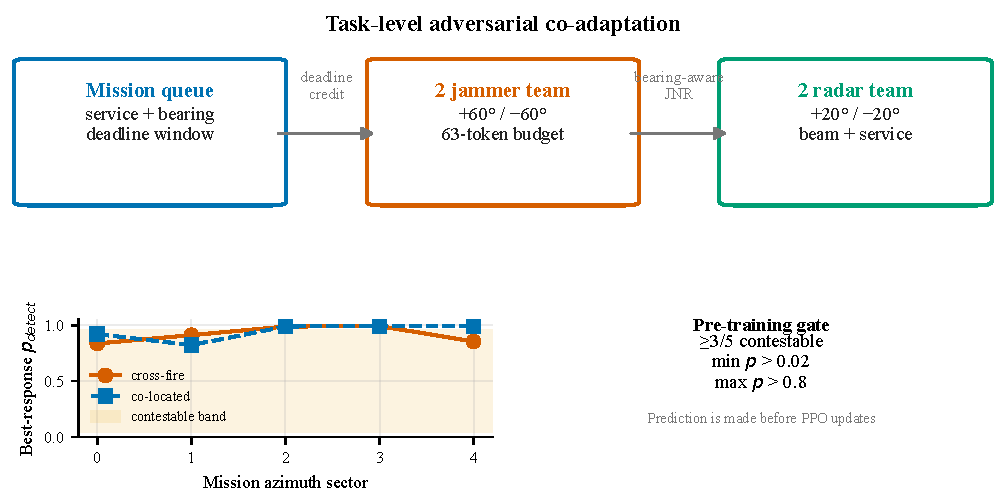
\includegraphics[width=0.96\textwidth]{figures/fig1_benchmark_anatomy.pdf}
\caption{Benchmark anatomy and pre-training contestability. FluxPhased couples a deadline-constrained mission queue to bearing-aware jammer--radar link physics. The lower panel reports the best-response detection profiles used to gate the cross-fire and co-located configurations before training.}
\label{fig:benchmark}
\end{figure*}
